\section*{Системная динамика}
\addcontentsline{toc}{section}{Системная динамика}
\subsection*{Модель развития социального стресса}
\addcontentsline{toc}{subsection}{Модель развития социального стресса}

\textbf{Задание:}\\
Реализовать и проанализировать модель развития социального стресса.\\

\textbf{Решение:}\\
Имеется три фазы развития психологического стресса:
\begin{enumerate}[topsep=0pt,itemsep=-1ex,partopsep=1ex,parsep=1ex]
	\item начальная;
	\item генерализированная;
	\item восстановительная;
\end{enumerate}

\begin{align*}
	\begin{cases}
		\dfrac{dN_1}{dt} = -\alpha V N_1 N_2 - p V N_1 + q N_3\\[10pt]
		\dfrac{dN_2}{dt} = \alpha V N_1 N_2 + p V N_1 - \beta N_2\\[10pt]
		\dfrac{dN_3}{dt} = \beta N_2 - q N_3\\[10pt]
		\dfrac{dV}{dt} = (cN_1 -r - m_0) V\\
	\end{cases}
\end{align*}

V -- степень <<эмоциональной выраженности>> информации, обусловленной стрессовым фактором.\\

Механизмы психологического давления:
\begin{enumerate}[topsep=0pt,itemsep=-1ex,partopsep=1ex,parsep=1ex]
	\item $r = m \cdot N_3$
	\item $r = m \cdot N_2$
	\item $r = m \cdot (N_2 + N_3)$
\end{enumerate}

\newpage

Покажем поведение модели при начальных значениях $N_1(0) = 995$, $N_2(0) = 5$, $V(0) = 1$, $\alpha = 0.0005$, $q = 0.05$, $b = 1/15$, $c = 0.0001$, $m = 0.00005$, $m_0 = 0.05$, $H = 1000$, $p = 0.017$. (Рисунок \ref{fig:sysdynamic1})
\begin{figure}[h]
	\centering 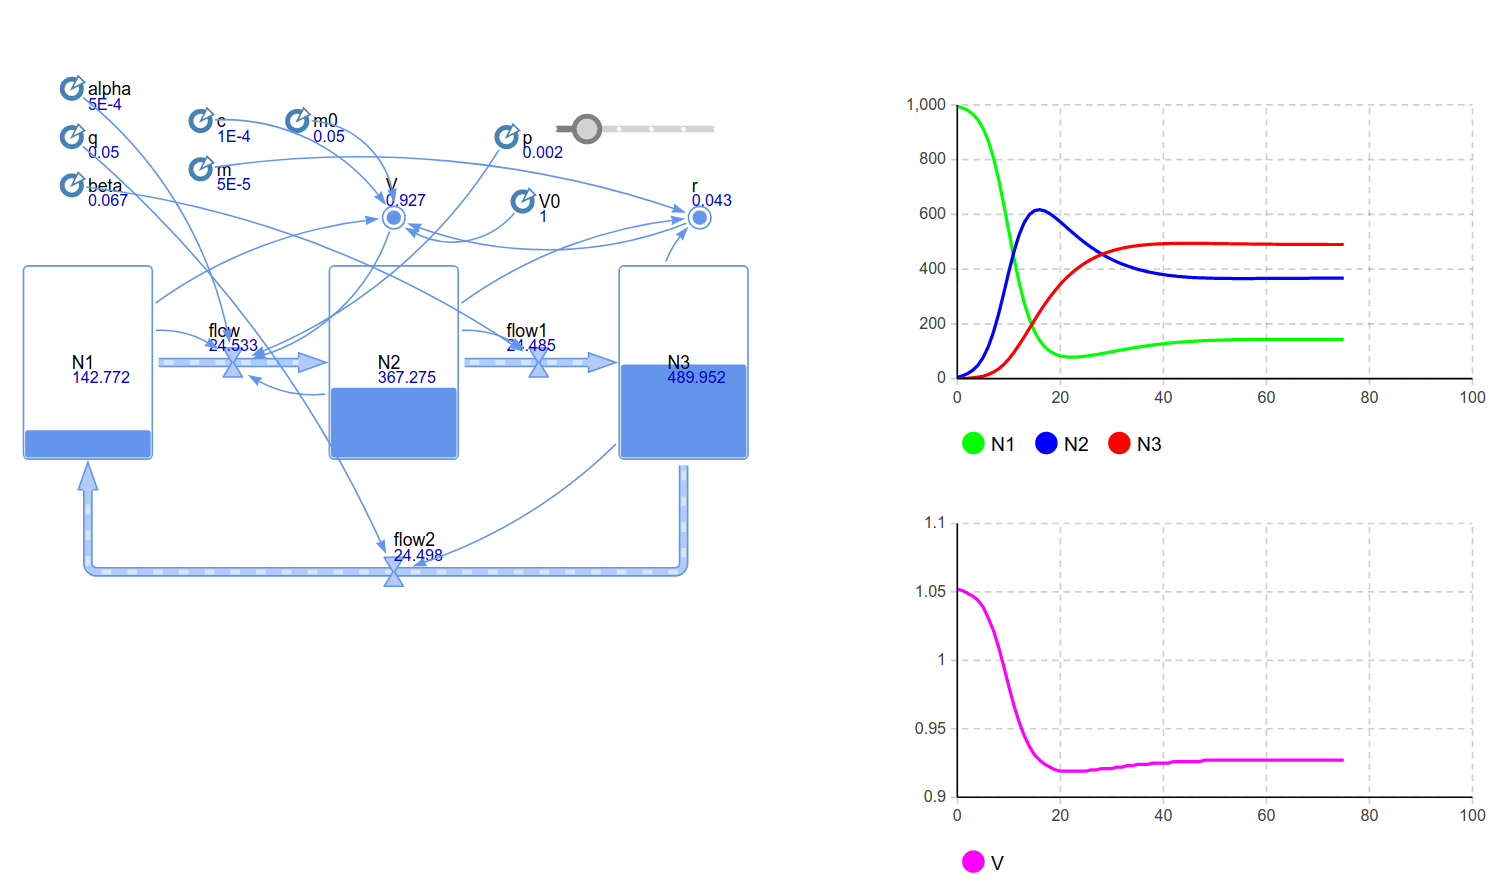
\includegraphics[scale=0.225]{sysdynamic1}
	\caption{Модель развития социального стресса при $p = 0.0017$}
	\label{fig:sysdynamic1}
\end{figure}

\begin{figure}[h]
	\centering 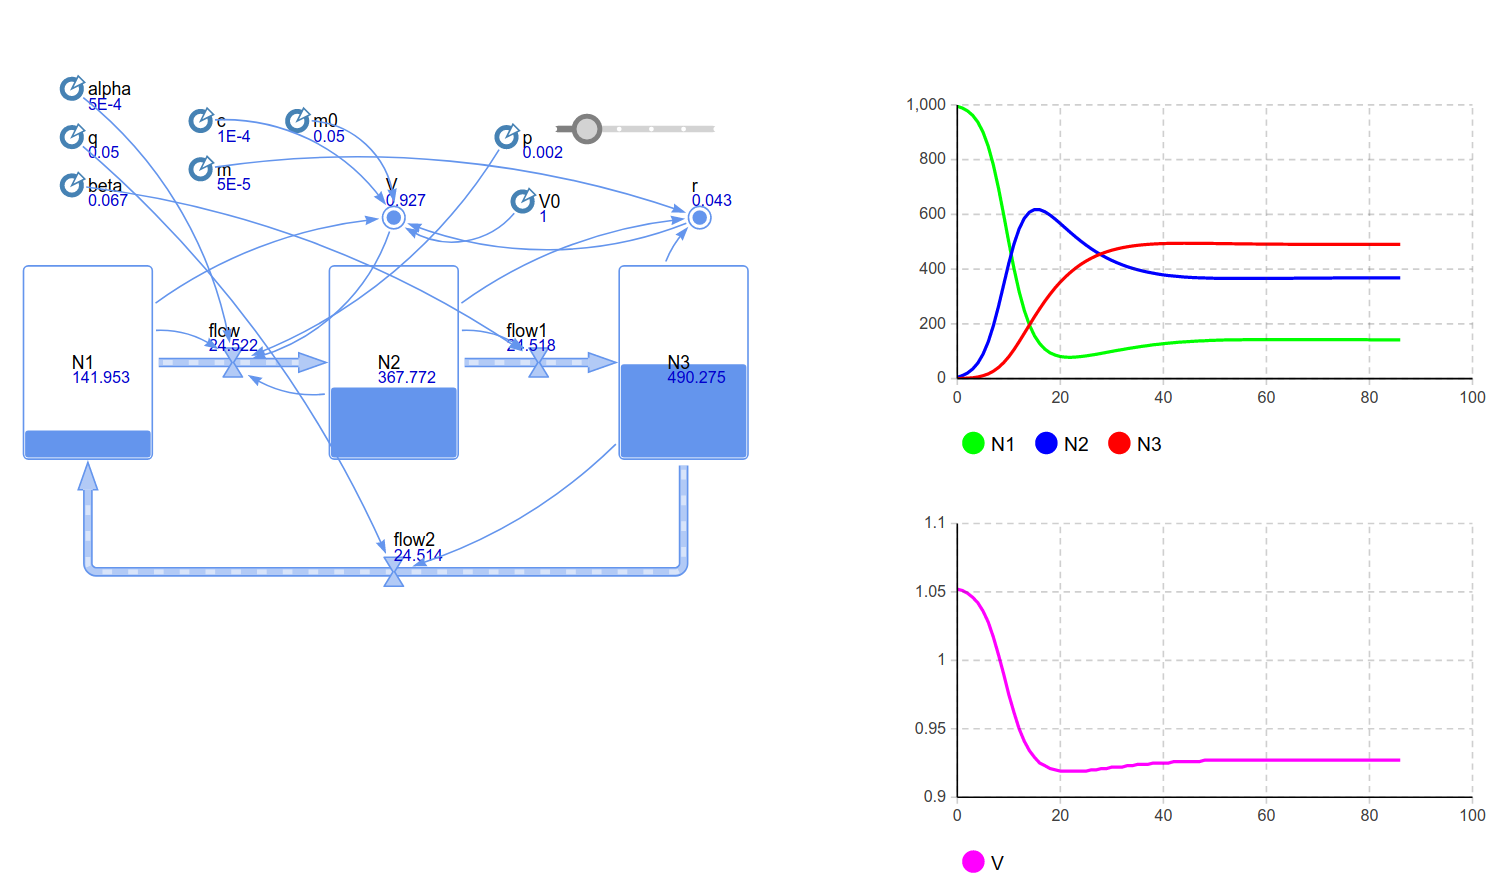
\includegraphics[scale=0.225]{sysdynamic2}
	\caption{Модель развития социального стресса при $p = 0.00246$}
	\label{fig:sysdynamic2}
\end{figure}

\newpage

\begin{figure}[h]
	\centering 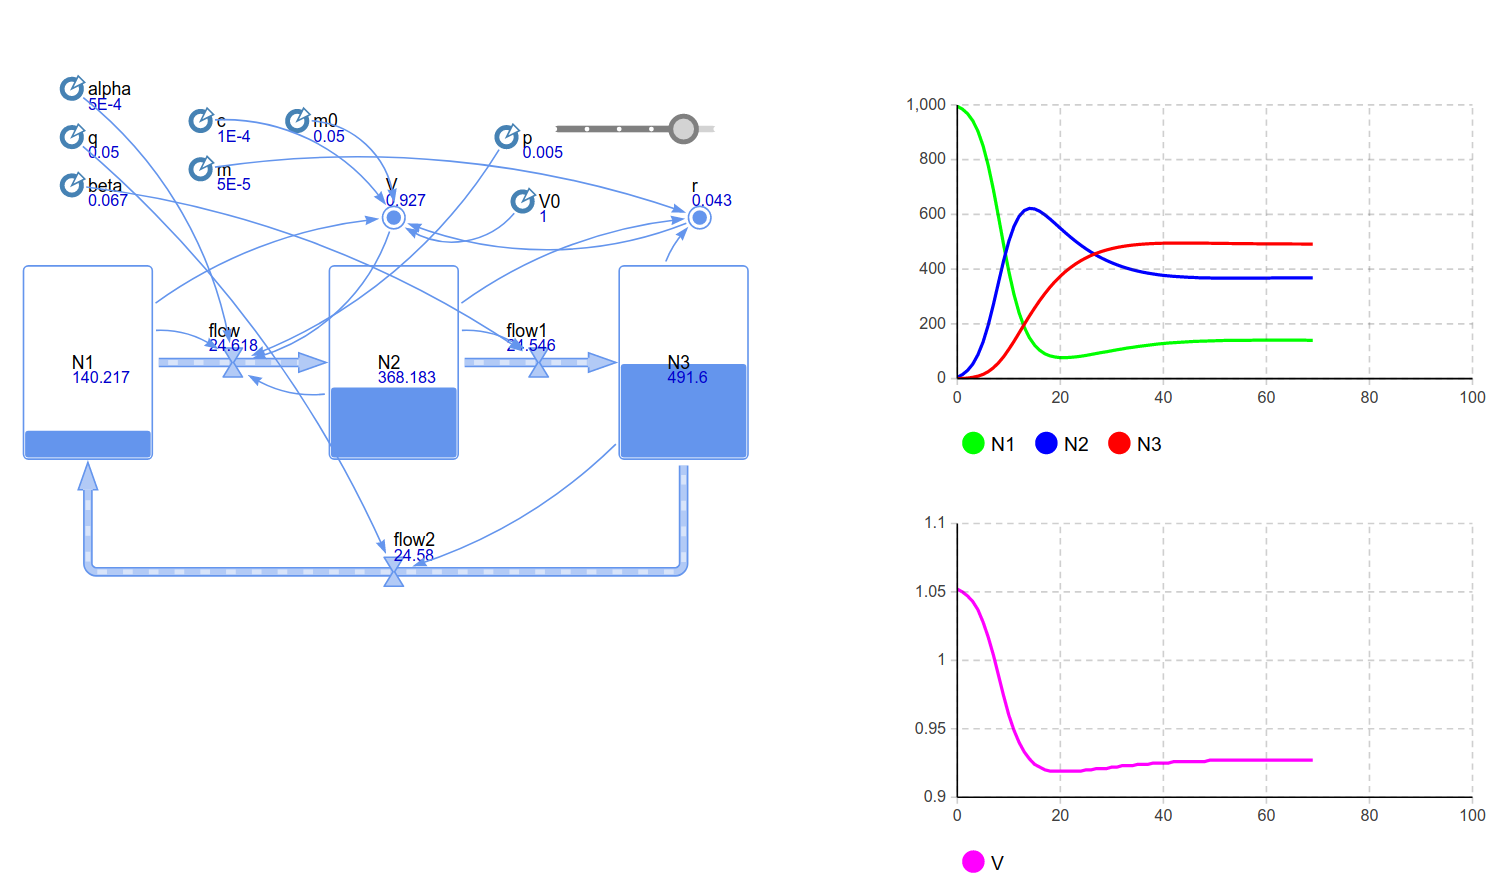
\includegraphics[scale=0.25]{sysdynamic3}
	\caption{Модель развития социального стресса при $p = 0.00534$}
	\label{fig:sysdynamic3}
\end{figure}

Из графиков можно видеть, что чем больше значение $p$, тем интенсивнее происходят изменения в составе групп. Также данная модель с течением времени приходит к станционарному состоянию из-за того, что $V$ примет значение, при котором численность групп будет оставаться на том же уровне.\\

Таким образом, можно вывести закономерность, связанную с изменением численности групп подверженных стрессу. С ростом степени <<эмоциональной выраженности>> информации, обусловленной стрессовыми факторами, увеличивается численность людей в генерализированной стадии, с ростом численности данной группы увеличивается численность людей в восстановительной стадии, с ростом численности данной группы уменьшается степень <<эмоциональной выраженности>>. С уменьшением степени <<эмоциональной выраженности>> возрастает численность людей в начальной стадии и уменьшается численность оставшихся групп.\\

Таким образом, была реализована модель развития социального стресса, был проведён численный анализ и были проанализированы взаимосвязи между переменными и параметрами модели.